%% ----------------------------------------------------------------------
%% START OF FILE
%% ----------------------------------------------------------------------

\chapter{系统测试和结果分析}
\label{cha:exp_analysis}

\section{实验平台}
\label{sec:exp_platform}

操作系统 Microsoft Windows Server 2008 R2

机械硬盘 250GB seagate st9250320as

固态硬盘 120GB crucial ct120m500ssd1

驱动程序开发工具 Microsoft Windows Driver Kit 7600.1

应用程序开发工具 Microsoft Visual Studio 2008

\section{实验方法}
\label{sec:exp_method}

\subsection{测试工具}
FIO是一款广泛使用的基于GPLv2协议的存储器性能评测工具,主要用来对存储设备进行性能验证和压力测试,也提供针对CPU和NIC的IO性能测试功能。FIO支持13种不同的IO引擎,可以通过多线程或多进程模拟各种IO操作。作为一款开源工具,FIO支持几乎所有常见的操作系统平台:Linux,FreeBSD,NetBSD,OS X,OpenSolaris,AIX以及Windows。

FIO只提供了与用户交互的命令行界面,由于提供了丰富的可配置的参数,FIO的可定制性非常强,可以根据测试者的想法进行各种混合IO的测试。本论文的系统测试也只使用了其中的小一部分参数。

\subsection{测试参数说明}

以下逐一介绍论文系统测试中所用到的FIO选项和具体参数说明。

\begin{lstlisting}
filename=\\\\.\\C:
\end{lstlisting}

filename参数指定了需要进行测试的设备文件。本论文实现的缓存系统以存储卷为单位,Windows操作系统只有将存储卷映射到某个的盘符(C、D、E……)后,才可进行访问。因此,对FIO来说要测试的存储设备指的就是某个盘符所映射的存储卷。

\begin{lstlisting}
size=2000MB
\end{lstlisting}

size参数指定待测试存储设备的空间大小,本论文测试的机械硬盘存储卷大小为2000MB。一般来说,缓存大小设定为存储空间大小的5\%-15\%,缓存系统对系统IO性能提升的贡献最为明显。因此,论文测试中将缓存卷的大小设定为200MB。缓存卷可使用系统自带的存储卷管理程序划分。

\begin{lstlisting}
iodepth=8
\end{lstlisting}

iodepth参数用来设定测试中并发的IO请求个数。应用程序通常使用同步和异步两种方式访问存储设备。以同步方式访问设备时,下一个IO请求要在上一个完成后才可进行,因此iodepth总是为1;异步方式访问,每次提交一批IO请求然后等这一批请求的完成,这样做可以减少交互的次数,让设备有机会合并IO请求以及进行内部的并行处理。在多进程的操作系统内,绝大多数情况下iodepth大于1。

\begin{lstlisting}
numjobs=4
\end{lstlisting}

numjobs参数设定了同时进行的负载个数,即每个线程产生一个负载进行测试,同时启动的线程个数。

\begin{lstlisting}
blocksize=[4k, 16k, 64k]
\end{lstlisting}

blocksize参数指定了测试时每个IO请求的大小,即每次读写的存储块大小,默认为4KB。本论文分别使用了4KB,16KB,64KB三种不同大小进行测试,以模拟不同应用场景下应用程序对于存储设备的读写请求,同时还可以评估设定的可变长缓存块大小对于缓存系统性能的影响。

\begin{lstlisting}
rw=[randrw, randread, randwrite]
\end{lstlisting}

rw参数设定每次测试所产生的读写类型。FIO提供了顺序读、顺序写、混合顺序读写、随机读、随机写、混合随机读写六种读写类型,每次测试只能选择一种类型。顺序读写的特性使得缓存系统难以达到理想的缓存命中率,因此本论文不进行顺序读写的测试,只测试随机读、随机写和混合随机读写三种读写类型。

\begin{lstlisting}
runtime=1000
\end{lstlisting}

runtime参数控制FIO运行多长时间后退出执行并给出测试结果,单位是秒。如果运行时间太短,测试结果受系统内其他进程影响,波动较大。经过多次实验,测试时间长1000秒时性能趋于稳定,此时的测试结果最有说服力。

\begin{lstlisting}
random_distribution=zipf:1.2
\end{lstlisting}

FIO提供random\_distribution参数配置访问设备文件一部分空间的概率,比其他部分的大,而并非平均分散到各处,从而获得存在热数据时的访问效果。默认情况下,读写位置的分布完全随机,此时测试出的缓存性能无法体现出真实情况下,热数据会被频繁访问的效果,缓存命中率也不具备说服力。论文测试中使用了齐夫分布这种概率分布模型,参数为1.2。

\section{实验结果}
\label{sec:exp_results}
论文实现的缓存系统可运行于写回和写穿两种模式,每种模式下需要进行随机读、随机写和混合随机读写三种读写类型的测试。

\subsection{缓存命中率}
\begin{table}[H]
\centering
\caption{写回、写穿两种模式下的缓存命中率}
\begin{tabular}{|c|c|c|c|}
\hline
\diagbox{模式}{测试类型} & 随机读 & 随机写 & 混合随机读写 \\ 
\hline 写穿模式 & 70.27\% & 70.75\% & 70.61\% \\ 
\hline 写回模式 & 76.29\% & 76.43\% & 73.64\% \\ 
\hline 
\end{tabular} 
\label{tab:cache-hit-rate}
\end{table}

\subsection{写穿(Write Through)策略时的测试结果}
\begin{itemize}

\item 随机读速度测试

\begin{table}[H]
\centering
\caption{随机读速度(KB/s,写穿法)}
\begin{tabular}{|c|c|c|c|}
\hline
\diagbox{块大小(KB)}{存储介质} & HDD & SSD & HDD with SSD Cache \\ 
\hline 4 & 417 & 19264 & 2063 \\ 
\hline 16 & 1651 & 59735 & 6319 \\ 
\hline 64 & 5810 & 142304 & 13203 \\ 
\hline 
\end{tabular} 
\label{tab:wt-rand-read-test}
\end{table}

写穿模式下,HDD的随机读性能有2.3-4.9倍的提升。

\item 随机写速度测试

\begin{table}[H]
\centering
\caption{随机写速度(KB/s,写穿法)}
\begin{tabular}{|c|c|c|c|}
\hline
\diagbox{块大小(KB)}{存储介质} & HDD & SSD & HDD with SSD Cache \\ 
\hline 4 & 1283 & 18620 & 1155 \\ 
\hline 16 & 5043 & 40634 & 4768 \\ 
\hline 64 & 16346 & 41615 & 15490 \\ 
\hline 
\end{tabular} 
\label{tab:wt-rand-write-test}
\end{table}

写穿模式下,由于没有对写操作进行缓存,HDD随机写的性能略差于无缓存情况下的写性能。

\item 随机读写:读速度测试

\begin{table}[H]
\centering
\caption{随机读写-读速度(KB/s,写穿法)}
\begin{tabular}{|c|c|c|c|}
\hline
\diagbox{块大小(KB)}{存储介质} & HDD & SSD & HDD with SSD Cache \\ 
\hline 4 & 420 & 14693 & 1590 \\ 
\hline 16 & 1657 & 46650 & 5327 \\ 
\hline 64 & 5598 & 105242 & 11929 \\ 
\hline 
\end{tabular} 
\label{tab:wt-randrw-read-test}
\end{table}

写穿模式下进行随机读写测试,HDD的随机读性能有2.1-3.7倍的提升。

\item 随机读写:写速度测试

\begin{table}[H]
\centering
\caption{随机读写-写速度(KB/s,写穿法)}
\begin{tabular}{|c|c|c|c|}
\hline
\diagbox{块大小(KB)}{存储介质} & HDD & SSD & HDD with SSD Cache \\ 
\hline 4 & 45 & 1688 & 181 \\ 
\hline 16 & 180 & 5427 & 616 \\ 
\hline 64 & 599 & 11925 & 1371 \\ 
\hline 
\end{tabular} 
\label{tab:wt-randrw-write-test}
\end{table}

写穿模式下进行随机读写测试,HDD的随机写性能有2.4-4.0倍的提升。

\end{itemize}

\subsection{写回(Write Back)策略时的测试结果}
\begin{itemize}

\item 随机读速度测试

\begin{table}[H]
\centering
\caption{随机读速度(KB/s,写回法)}
\begin{tabular}{|c|c|c|c|}
\hline
\diagbox{块大小(KB)}{存储介质} & HDD & SSD & HDD with SSD Cache \\ 
\hline 4 & 417 & 19264 & 2970 \\ 
\hline 16 & 1651 & 59735 & 9821 \\ 
\hline 64 & 5810 & 142304 & 32857 \\ 
\hline 
\end{tabular} 
\label{tab:wb-rand-read-test}
\end{table}

写回模式下,HDD的随机读性能有5.6-7.1倍的提升。

\item 随机写速度测试

\begin{table}[H]
\centering
\caption{随机写速度(KB/s,写回法)}
\begin{tabular}{|c|c|c|c|}
\hline
\diagbox{块大小(KB)}{存储介质} & HDD & SSD & HDD with SSD Cache \\ 
\hline 4 & 1283 & 18620 & 3459 \\ 
\hline 16 & 5043 & 40634 & 8697 \\ 
\hline 64 & 16346 & 41615 & 21794 \\ 
\hline 
\end{tabular} 
\label{tab:wb-rand-write-test}
\end{table}

写回模式下,HDD的随机写性能有1.3-2.6倍的提升。

\item 随机读写:读速度测试

\begin{table}[H]
\centering
\caption{随机读写-读速度(KB/s,写回法)}
\begin{tabular}{|c|c|c|c|}
\hline
\diagbox{块大小(KB)}{存储介质} & HDD & SSD & HDD with SSD Cache \\ 
\hline 4 & 420 & 14693 & 2725 \\ 
\hline 16 & 1657 & 46650 & 8693 \\ 
\hline 64 & 5598 & 105242 & 27696 \\ 
\hline 
\end{tabular} 
\label{tab:wb-randrw-read-test}
\end{table}

写回模式下进行随机读写测试,HDD的随机读性能有4.9-6.4倍的提升。

\item 随机读写:写速度测试

\begin{table}[H]
\centering
\caption{随机读写-写速度(KB/s,写回法)}
\begin{tabular}{|c|c|c|c|}
\hline
\diagbox{块大小(KB)}{存储介质} & HDD & SSD & HDD with SSD Cache \\ 
\hline 4 & 45 & 1688 & 309 \\ 
\hline 16 & 180 & 5427 & 985 \\ 
\hline 64 & 599 & 11925 & 3221 \\ 
\hline 
\end{tabular} 
\label{tab:wb-randrw-write-test}
\end{table}

写回模式下进行随机读写测试,HDD的随机写性能有5.3-6.8倍的提升。

\end{itemize}

\section{结果与讨论}
\label{sec:results_and_comparation}

\subsection{HDD性能提升比例}

\begin{figure}[H]
\centering
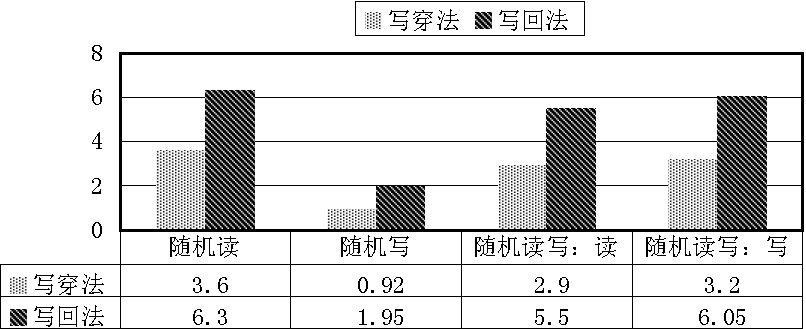
\includegraphics[width=0.9\linewidth]{./graph/enhance-rate}
\caption{读写性能提升比例比较}
\label{fig:enhance-rate}
\end{figure}

从图\ref{fig:enhance-rate}可以看出,由于缓存系统的存在,HDD的随机读、随机写性能都得到了一定程度的提升。相较于写穿法,写回法对存储系统总体性能提升的比例更为明显。

\subsection{与FancyCache软件比较}
FancyCache是一款使用SSD作为缓存提升存储系统性能的商业软件。FancyCache可以将系统内存或SSD空间设置成机械硬盘的缓存。该软件将从硬盘中读取的数据存入系统内存或闪存,使系统在下次访问该数据时可以很快从内存读取,避免再次读取速度较慢的硬盘,从而突破硬盘瓶颈,提升系统性能。FancyCache还具有检测和利用系统未识别内存的功能,解决32位Windows操作系统无法完全使用4G或更多内存的问题。通过将检测到的系统未识别内存用作硬盘缓存的方式,FancyCache能够使用32位操作系统无法识别出的物理内存。

为了说明本论文实现的缓存系统与主流缓存软件对系统性能提升的差距,在系统的实验阶段,论文还测试了使用FancyCache缓存软件时的读写性能提升。由于通过上节的测试可以得出本论文实现的缓存系统运行于回写模式时,对HDD的随机读写性能提升最为明显,且FancyCache的缓存也是运行于回写模式,所以本节会使用运行于回写模式时HDD的随机读写性能和FancyCache软件进行比较。

\begin{table}[H]
\centering
\caption{随机读速度比较(KB/s)}
\begin{tabular}{|c|c|c|}
\hline
\diagbox{块大小(KB)}{缓存系统} & 本论文的 & FancyCache \\ 
\hline 4  & 2970 & 2508 \\ 
\hline 16 & 9821 & 10254 \\ 
\hline 64 & 32857 & 51833 \\ 
\hline 
\end{tabular} 
\label{tab:wb-rand-read-comp}
\end{table}

从随机读测试的结果可以看出,IO请求的大小为4KB时,本论文实现的缓存系统性能优于FancyCache;当IO请求比较大时,FancyCache的效果更为明显,这是因为论文实现的缓存系统的缓存块单位是4KB,读写请求大于4KB时会将一个读写请求分为多个处理,影响了系统的性能。

\begin{table}[H]
\centering
\caption{随机写速度比较(KB/s)}
\begin{tabular}{|c|c|c|}
\hline
\diagbox{块大小(KB)}{缓存系统} & 本论文的 & FancyCache \\ 
\hline 4  & 2970 & 3021 \\ 
\hline 16 & 9821 & 9982 \\ 
\hline 64 & 32857 & 32258 \\ 
\hline 
\end{tabular} 
\label{tab:wb-rand-write-comp}
\end{table}

进行随机写测试,IO请求的大小为4KB和16KB时,FancyCache的性能优于本论文实现的缓存系统,但差距不大;IO请求的大小为64KB时,本论文实现的缓存系统略优于FancyCache。

%% ----------------------------------------------------------------------
%%% END OF FILE
%% ----------------------------------------------------------------------
